\documentclass[]{book}
\usepackage{lmodern}
\usepackage{amssymb,amsmath}
\usepackage{ifxetex,ifluatex}
\usepackage{fixltx2e} % provides \textsubscript
\ifnum 0\ifxetex 1\fi\ifluatex 1\fi=0 % if pdftex
  \usepackage[T1]{fontenc}
  \usepackage[utf8]{inputenc}
\else % if luatex or xelatex
  \ifxetex
    \usepackage{mathspec}
  \else
    \usepackage{fontspec}
  \fi
  \defaultfontfeatures{Ligatures=TeX,Scale=MatchLowercase}
\fi
% use upquote if available, for straight quotes in verbatim environments
\IfFileExists{upquote.sty}{\usepackage{upquote}}{}
% use microtype if available
\IfFileExists{microtype.sty}{%
\usepackage{microtype}
\UseMicrotypeSet[protrusion]{basicmath} % disable protrusion for tt fonts
}{}
\usepackage[margin=1in]{geometry}
\usepackage{hyperref}
\hypersetup{unicode=true,
            pdftitle={Vol. 0: Basics in R},
            pdfauthor={Sarah Schwartz \& Tyson Barrett},
            pdfborder={0 0 0},
            breaklinks=true}
\urlstyle{same}  % don't use monospace font for urls
\usepackage{natbib}
\bibliographystyle{apalike}
\usepackage{longtable,booktabs}
\usepackage{graphicx,grffile}
\makeatletter
\def\maxwidth{\ifdim\Gin@nat@width>\linewidth\linewidth\else\Gin@nat@width\fi}
\def\maxheight{\ifdim\Gin@nat@height>\textheight\textheight\else\Gin@nat@height\fi}
\makeatother
% Scale images if necessary, so that they will not overflow the page
% margins by default, and it is still possible to overwrite the defaults
% using explicit options in \includegraphics[width, height, ...]{}
\setkeys{Gin}{width=\maxwidth,height=\maxheight,keepaspectratio}
\IfFileExists{parskip.sty}{%
\usepackage{parskip}
}{% else
\setlength{\parindent}{0pt}
\setlength{\parskip}{6pt plus 2pt minus 1pt}
}
\setlength{\emergencystretch}{3em}  % prevent overfull lines
\providecommand{\tightlist}{%
  \setlength{\itemsep}{0pt}\setlength{\parskip}{0pt}}
\setcounter{secnumdepth}{5}
% Redefines (sub)paragraphs to behave more like sections
\ifx\paragraph\undefined\else
\let\oldparagraph\paragraph
\renewcommand{\paragraph}[1]{\oldparagraph{#1}\mbox{}}
\fi
\ifx\subparagraph\undefined\else
\let\oldsubparagraph\subparagraph
\renewcommand{\subparagraph}[1]{\oldsubparagraph{#1}\mbox{}}
\fi

%%% Use protect on footnotes to avoid problems with footnotes in titles
\let\rmarkdownfootnote\footnote%
\def\footnote{\protect\rmarkdownfootnote}

%%% Change title format to be more compact
\usepackage{titling}

% Create subtitle command for use in maketitle
\newcommand{\subtitle}[1]{
  \posttitle{
    \begin{center}\large#1\end{center}
    }
}

\setlength{\droptitle}{-2em}

  \title{Vol. 0: Basics in R}
    \pretitle{\vspace{\droptitle}\centering\huge}
  \posttitle{\par}
    \author{Sarah Schwartz \& Tyson Barrett}
    \preauthor{\centering\large\emph}
  \postauthor{\par}
      \predate{\centering\large\emph}
  \postdate{\par}
    \date{Last updated: 2018-08-13}

\usepackage{booktabs}
\usepackage{amsthm}
\makeatletter
\def\thm@space@setup{%
  \thm@preskip=8pt plus 2pt minus 4pt
  \thm@postskip=\thm@preskip
}
\makeatother

\begin{document}
\maketitle

{
\setcounter{tocdepth}{1}
\tableofcontents
}
\chapter{Introduction}\label{introduction}

\textbf{What is R?}

R is a language and environment for statistical computing and graphics.
\citep{R-base}

R provides a wide variety of statistical (linear and nonlinear
modelling, classical statistical tests, time-series analysis,
classification, clustering, \ldots{}) and graphical techniques, and is
highly extensible. The S language is often the vehicle of choice for
research in statistical methodology, and R provides an Open Source route
to participation in that activity.

One of R's strengths is the ease with which well-designed
publication-quality plots can be produced, including mathematical
symbols and formulae where needed. Great care has been taken over the
defaults for the minor design choices in graphics, but the user retains
full control.

\textbf{What is R Markdown?}

According to \href{www.rstudio.com}{R Studio}:

\begin{quote}
``R Markdown is a format that enables easy authoring of reproducible web
reports from R. It combines the core syntax of Markdown (an
easy-to-write \textbf{plain text} format for web content) with embedded
\textbf{R code chunks} that are run so their output can be included in
the final document''.
\end{quote}

\begin{center}\rule{0.5\linewidth}{\linethickness}\end{center}

\textbf{Dynamic Reporting}

From
\href{https://onlinecourses.science.psu.edu/statprogram/markdown}{Penn
State Statistics}:

\textbf{The }traditional way** to write a report**

\begin{enumerate}
\def\labelenumi{\arabic{enumi}.}
\tightlist
\item
  Run your analysis in software, like SPSS or R and manually save our
  output

  \begin{itemize}
  \tightlist
  \item
    \emph{i.e.~saving the ANOVA table or using pdf() to save the graphs}
  \end{itemize}
\item
  Type your your description and interpretation in a text editor like
  \emph{Word}

  \begin{itemize}
  \tightlist
  \item
    \emph{either drag/drop tables and figures, or worse copy-paste and
    retype all the numbers}
  \end{itemize}
\end{enumerate}

A report written in this way can be problematic. For instance, imagine
your \emph{Mentor/collaborator/journal reviewer} telling you that they
want to use a sub-sample instead of the entire sample. Or to include a
nother variable. You would have to redo all of your work!!

Therefore, in this way \textbf{dynamic also means reproducible}, in the
sense that people who get the file from you can reproduce the entire
work in the report.

\textbf{How does R Markdown work out to be a .pdf or .html file?}

\texttt{R\ Markdown} is a file with the file extension \textbf{.Rmd},
the \texttt{knitr} package will then transform the file into a
\textbf{Markdown} file with the extension \textbf{.md.} Then Rstudio can
\citep{xie2015}:

\begin{itemize}
\item
  Use \texttt{LaTeX} to transform the file into a \textbf{.pdf}
\item
  Load another package called \texttt{markdown} to transform the file
  into \textbf{.html}
\item
  Use Pandoc to even convert to file to a \textbf{Word} document (ugly)
\end{itemize}

\textbf{Is this a }popular** method for creating reports?**

Check out \href{http://rpubs.com/}{Rpubs}. This website shares lots of
documents written in the way we will introduce below.

\begin{figure}
\centering
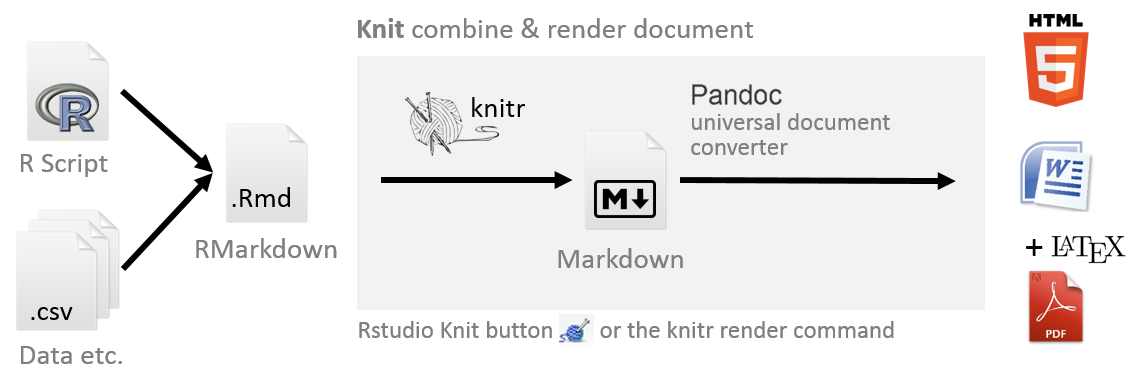
\includegraphics{img/processRStudio.png}
\caption{}
\end{figure}

\begin{center}\rule{0.5\linewidth}{\linethickness}\end{center}

\begin{figure}
\centering

\includegraphics{img/hex/rmarkdown-200x232.png}
\caption{}
\end{figure}

\begin{quote}
\texttt{R\ Markdown} documents are fully reproducible. Use a productive
\textbf{notebook} interface to weave together narrative text and code to
produce elegantly formatted output. Use multiple languages including R,
Python, and SQL \citep{R-rmarkdown}.
\end{quote}

\begin{figure}
\centering

\includegraphics{img/hex/knitr-200x232.png}
\caption{}
\end{figure}

\begin{quote}
\texttt{knitr} is an engine for dynamic report generation with R. It is
a package in the statistical programming language R that enables
integration of \textbf{R code} into LaTeX, LyX, HTML, Markdown,
AsciiDoc, and \textbf{text} documents \citep{R-knitr}.
\end{quote}

\chapter{Software Installation}\label{software-installation}

Here is where we talk about installing software.

\begin{center}\rule{0.5\linewidth}{\linethickness}\end{center}

\section{R}\label{r}

\subsection{First Time Installation}\label{first-time-installation}

\subsection{Periotic Updating}\label{periotic-updating}

\begin{center}\rule{0.5\linewidth}{\linethickness}\end{center}

\section{R Studio}\label{r-studio}

\subsection{First Time Installation}\label{first-time-installation-1}

\subsection{Periotic Updating}\label{periotic-updating-1}

\subsection{Panel Layout}\label{panel-layout}

\begin{center}\rule{0.5\linewidth}{\linethickness}\end{center}

\section{TeX (optional)}\label{tex-optional}

\subsection{TinyTeX}\label{tinytex}

\subsection{MAc}\label{mac}

\subsection{Windows}\label{windows}

\chapter{Packages Management}\label{packages-management}

We describe packages and their management

\begin{center}\rule{0.5\linewidth}{\linethickness}\end{center}

\section{What are packages}\label{what-are-packages}

\begin{center}\rule{0.5\linewidth}{\linethickness}\end{center}

\section{How to install packages}\label{how-to-install-packages}

\begin{center}\rule{0.5\linewidth}{\linethickness}\end{center}

\section{Updating packages}\label{updating-packages}

\begin{center}\rule{0.5\linewidth}{\linethickness}\end{center}

\section{Suggested packages}\label{suggested-packages}

\chapter{Data Management}\label{data-management}

How do you get data into R, view and work with in, and then save it for
later use.

\begin{center}\rule{0.5\linewidth}{\linethickness}\end{center}

\section{Importing Data From Various
Formats}\label{importing-data-from-various-formats}

\subsection{Text Format (.csv, tab-delimited,
ect.)}\label{text-format-.csv-tab-delimited-ect.}

Use \texttt{read.csv()}

\subsection{Excel Format (.xls, .xlsx)}\label{excel-format-.xls-.xlsx}

Use \texttt{haven::read.spss()}

\subsection{SPSS Format (.sav)}\label{spss-format-.sav}

Use \texttt{readxl::read.excel()}

\subsection{REDCap (API directly)}\label{redcap-api-directly}

\begin{center}\rule{0.5\linewidth}{\linethickness}\end{center}

\section{Viewing Data Within R
Studio}\label{viewing-data-within-r-studio}

\subsection{The Environment Tab}\label{the-environment-tab}

\subsection{Notebook Display}\label{notebook-display}

\begin{center}\rule{0.5\linewidth}{\linethickness}\end{center}

\section{Saving Data in R Format}\label{saving-data-in-r-format}

Use \texttt{save(...,\ file\ =\ "name.RData")}

\chapter{Data Wrangling}\label{data-wrangling}

\begin{center}\rule{0.5\linewidth}{\linethickness}\end{center}

\section{Subseting Data}\label{subseting-data}

\subsection{Select Variables (columns)}\label{select-variables-columns}

Use \texttt{dplyr::select()}

\subsection{Select Observations (rows)}\label{select-observations-rows}

Use \texttt{dplyr::filter()}

\begin{center}\rule{0.5\linewidth}{\linethickness}\end{center}

\section{Symbol Opporators}\label{symbol-opporators}

\subsection{Logical Opporators}\label{logical-opporators}

\subsubsection{\texorpdfstring{Ineqalities (\texttt{\textless{}},
\texttt{\textgreater{}}, \texttt{\textless{}=},
\texttt{\textless{}=})}{Ineqalities (\textless{}, \textgreater{}, \textless{}=, \textless{}=)}}\label{ineqalities}

\subsubsection{\texorpdfstring{AND ( \texttt{\&}
)}{AND ( \& )}}\label{and}

\subsubsection{\texorpdfstring{OR
(\texttt{\textbar{}})}{OR (\textbar{})}}\label{or}

\subsubsection{\texorpdfstring{Within a List ( \texttt{\%in\%}
)}{Within a List ( \%in\% )}}\label{within-a-list-in}

\subsection{\texorpdfstring{The Assignemnt Opporator (
\texttt{\textless{}-}
)}{The Assignemnt Opporator ( \textless{}- )}}\label{the-assignemnt-opporator--}

\subsection{\texorpdfstring{The Pipe Opporator (
\texttt{\%\textgreater{}\%}
)}{The Pipe Opporator ( \%\textgreater{}\% )}}\label{the-pipe-opporator}

\bibliography{book.bib,packages.bib}


\end{document}
